\documentclass[letterpaper,12pt,fleqn]{article}
\usepackage{matharticle}
\usepackage{mathtools}
\usepackage{tikz}
\renewcommand{\o}{\theta}
\pagestyle{plain}
\begin{document}

\begin{center}
\Large Math-19 Homework \#8
\end{center}

\vspace{0.5in}

\underline{Reading}

Please read sections 5.4-5.6 and 6.4-6.6, then do all concept problems in the
posted sections on web\-assign.

\underline{Problems}

\begin{enumerate}
\item Consider the function:
\[f(x)=2\tan(4\pi x-\pi)+1\]
\begin{enumerate}
\item What is the period $P$?
\item What is the horizontal translation $b$?
\item What is the phase angle $\phi$?
\item What is the y-intercept?
\item Sketch one cycle of the graph in the interval $(b,b+P)$ and then extend
the sketch back to the y-intercept.
\end{enumerate}

\item Solve for $x$:
\[\tan\left(3x+\frac{\pi}{2}\right)\sin(2\pi x)\cos(6x+\pi)=0\]
Hint: be careful about domain!

\item Two $1kg$ masses are each suspended on a spring with $k=\pi^2$ and are
stretched downward by 2 units. The first spring is released at $t=0$. The
second spring is released at $t=3$.
\begin{enumerate}
\item Find $f_1(t)$ for the first mass.
\item Find $f_2(t)$ for the second mass.
\item What is the phase difference between the two masses?
\end{enumerate}

\item Evaluate:
\[\cot\left(\cos^{-1}\frac{x}{\sqrt{1+x^2}}\right)\]
\newpage
\item Consider the following triangle:

\bigskip

\begin{figure}[h]
\setlength{\leftskip}{0.5in}
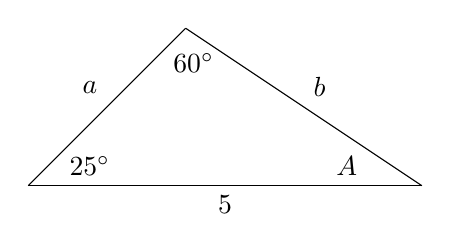
\begin{tikzpicture}
\draw (0,0) -- (5,0);
\draw (0,0) -- (2,2);
\draw (5,0) -- (2,2);
\node [below] at (2.5,0) {$5$};
\node [left] at (1,1.25) {$a$};
\node [right] at (3.5,1.25) {$b$};
\node [below] at (2.1,1.8) {$60^{\circ}$};
\node [above right] at (0.4,0) {$25^{\circ}$};
\node [above left] at (4.3,0) {$A$};
\end{tikzpicture}
\end{figure}

\begin{enumerate}
\item Determine $A$.
\item Determine $a$.
\item Determine $b$.
\item Using Heron's Formula, determine the area of the triangle.
\end{enumerate}
\end{enumerate}
\end{document}
